\chapter{ Método Propuesto }
Este trabajo propone una solución para determinar los momentos en los que se disparará la ejecución de los procesos de desfragmentación de manera proactiva en redes MC-EON, mediante la utilización de técnicas de \textit{Machine Learning} para predecir el índice de fragmentación \textit{\textbf{BFR}} que sufrirá la red mediante el tráfico de red en un determinado periodo de tiempo \textit{t} y en base a eso, decidir si ejecutar la desfragmentación o no.
 Esto a fin de proceder de la mejor manera ante la red cuando llegue a un estado de alta fragmentación que provoque un aumento en la probabilidad de bloqueo de las demandas y que la desfragmentación de la red en ese punto ya no sea óptima.
%

Para esta predicción se utiliza primeramente un valor que indique el umbral del indice de fragmentación, a modo que el valor predicho del índice de fragmentación a futuro no supere ese umbral, en caso contrario realizar las desfragmentaciones con menor frecuencia hasta que el indice de fragmentación futuro \textit{\textbf{BFR}} sea menor al umbral.
 Así como tambien un modelo de regresión y clasificación, utilizando un conjunto de datos de simulaciones de tráfico \textit{unicast}, tomando parámetros o características relacionadas a la fragmentación, la utilización de la red y las métricas específicas de múltiples núcleos como datos de entrada, produciendo un valor estimado del índice de fragmentación que experimentará la red en un periodo de tiempo \textit{t}.
  A partir de este valor predicho, se determinará la frecuencia de desfragmentaciones realizadas fijando un umbral que permite actuar antes de que la red alcance estados críticos de fragmentación que incrementen significativamente la probabilidad de bloqueo de las demandas.
%

\section{Características}

En el área de \textit{Machine Learning}, se conoce como ``características'' a los parámetros o datos de entrada del modelo de aprendizaje.

Las características seleccionadas fueron aquellas relacionadas al uso y la fragmentación de la red, así como métricas específicas de redes MC-EON. Se tomaron las principales métricas utilizadas para la determinación del estado de fragmentación, además de otras relacionadas a la utilización de la red y al comportamiento del tráfico, con el objetivo de predecir el índice de fragmentación futuro y determinar los momentos óptimos para ejecutar la desfragmentación de manera proactiva.

Estas características son las siguientes: 

\begin{itemize}
    \item \textit{Bandwidth Fragmentation Ratio} o Relación de Fragmentación de ancho de banda (BFR)\cite{zhang2013bandwidth}: Representa el índice de fragmentación de los recursos de la red, siendo una de las métricas principales para evaluar la fragmentación externa. El BFR de un core en un enlace se define como:
    \begin{equation}
        BFR_{core} = 1 - \frac{MaxBlock()}{S^{free}}
    \end{equation}
    Donde \textit{MaxBlock()} es el tamaño del mayor bloque de FS libres y \(S^{free}\) es la sumatoria total de FS libres en el core.
    El BFR de la red se calcula como el promedio ponderado considerando todos los cores de todos los enlaces:
    \begin{equation}
       BFR_{red} = 1 - \frac{\sum_{i=1}^{\left | E \right |} \sum_{j=1}^{C} MaxBlock_{i,j}}{\sum_{i=1}^{\left | E \right |} \sum_{j=1}^{C} S^{free}_{i,j}}
    \end{equation}
    Donde \(C\) es el número de cores por enlace, \(MaxBlock_{i,j}\) es el mayor bloque libre en el core \(j\) del enlace \(i\), y \(S^{free}_{i,j}\) es el total de FS libres en ese core.
    
    \item Entropía de Shannon (SHF)\cite{wright2015minimum}: Métrica de fragmentación que mide la distribución de bloques libres en el espectro. Para un core en un enlace está definida por:
    \begin{equation}
        SHF_{core} = \sum_{i=1}^{B} \frac{S_{i}^{free}}{N}~\ln\frac{N}{S_{i}^{free}}
    \end{equation}
    Donde \(S_{i}^{free}\) representa el tamaño del bloque libre \(i\), \(N\) es el número total de FS en el core, y \(B\) es la cantidad de bloques de FS libres. Para calcular el SHF de la red se calcula el promedio de los valores en todos los cores de todos los enlaces:
    \begin{equation}
        SHF_{red} = \frac{1}{\left | E \right | \times C} \sum_{i=1}^{\left | E \right |} \sum_{j=1}^{C} SHF_{core_{i,j}}
    \end{equation}
    
    \item Compacidad del Espectro (SC - \textit{Spectrum Compactness}): Métrica que evalúa qué tan compacto está el uso del espectro en un core. Se calcula considerando la dispersión de los FS ocupados y la cantidad de gaps intermedios. Para un core en un enlace se define como:
    \begin{equation}
        SC_{core} = \frac{s_{max} - s_{min} + 1}{S^{occupied}} \times \frac{\sum_{i=1}^{G} g_i}{G}
    \end{equation}
    Donde \(s_{min}\) y \(s_{max}\) son los índices del primer y último FS ocupado respectivamente, \(S^{occupied}\) es la cantidad total de FS ocupados, \(g_i\) es el tamaño del gap libre \(i\), y \(G\) es la cantidad total de gaps entre bloques ocupados. Si no hay FS ocupados, \(SC_{core} = 0\).
    El SC de la red se calcula como:
    \begin{equation}
        SC_{red} = \frac{1}{\left | E \right | \times C} \sum_{i=1}^{\left | E \right |} \sum_{j=1}^{C} SC_{core_{i,j}}
    \end{equation}
    
    \item \textit{Golden Metric} (GM): Métrica avanzada que evalúa la fragmentación considerando rangos de tamaño de demandas esperadas. Dado dos parámetros \(n_1\) y \(n_2\) que representan el rango de tamaños de demanda típicos, el GM para un core se calcula como:
    \begin{equation}
        GM_{core} = \frac{a}{|b|}
    \end{equation}
    Donde los valores de \(a\) y \(b\) se calculan iterando sobre cada gap de FS libres de tamaño \(g\):
    \begin{equation}
        a_0 = \epsilon, \quad b_0 = -\epsilon
    \end{equation}
    \begin{equation}
        a = a_0 + \sum_{i=1}^{G} a_i, \quad b = b_0 + \sum_{i=1}^{G} b_i
    \end{equation}
    Donde \(\epsilon = 0.001\) y para cada gap \(g_i\):
    \begin{itemize}
        \item Si \(g_i < n_1\): \(a_i = 0\), \(b_i = -\frac{g_i}{avg}\)
        \item Si \(g_i > n_2\): \(a_i = \frac{g_i}{avg}\), \(b_i = 0\)
        \item Si \(n_1 \leq g_i \leq n_2\): \(a_i = \frac{g_i - n_1 + 1}{avg}\), \(b_i = -\frac{n_2 - g_i}{avg}\)
    \end{itemize}
    Con \(avg = \frac{n_1 + n_2}{2}\).
    El GM de la red se calcula como:
    \begin{equation}
        GM_{red} = \frac{1}{\left | E \right | \times C} \sum_{i=1}^{\left | E \right |} \sum_{j=1}^{C} GM_{core_{i,j}}
    \end{equation}
    
    \item \textit{Available Spectrum Fragmentation Ratio 3D} (ASFR3D): Métrica que considera la fragmentación espacial en redes multi-core, evaluando bloques pequeños que no pueden ser utilizados eficientemente. Para un core se define como:
    \begin{equation}
        ASFR3D_{core} = \left(1 - \frac{S^{small}}{S^{free}}\right) \times F_{spatial}
    \end{equation}
    Donde \(S^{small}\) es la suma de FS libres en bloques menores a 5 slots, \(S^{free}\) es el total de FS libres, y \(F_{spatial}\) es un factor de peso espacial definido como:
    \begin{equation}
        F_{spatial} = \frac{\ln(D_{active} + 1)}{10}
    \end{equation}
    Donde \(D_{active}\) es el número de demandas activas en la red.
    El ASFR3D de la red se calcula como:
    \begin{equation}
        ASFR3D_{red} = \frac{1}{\left | E \right | \times C} \sum_{i=1}^{\left | E \right |} \sum_{j=1}^{C} ASFR3D_{core_{i,j}}
    \end{equation}
    
    \item Utilización Diferencial (UD): Métrica que mide el desbalance en la utilización entre diferentes cores y enlaces de la red. Se define como:
    \begin{equation}
        UD_{red} = U_{max} - U_{min}
    \end{equation}
    Donde \(U_{max}\) y \(U_{min}\) son las utilizaciones máxima y mínima entre todos los cores de todos los enlaces, siendo la utilización de un core:
    \begin{equation}
        U_{core} = \frac{S^{occupied}}{N}
    \end{equation}
    Con \(S^{occupied}\) siendo el número de FS ocupados y \(N\) el número total de FS en el core. Un valor alto de UD indica desbalance en la carga de la red, mientras que un valor bajo indica una distribución uniforme.
    
\end{itemize}

\begin{figure}[!h]
    \centering
    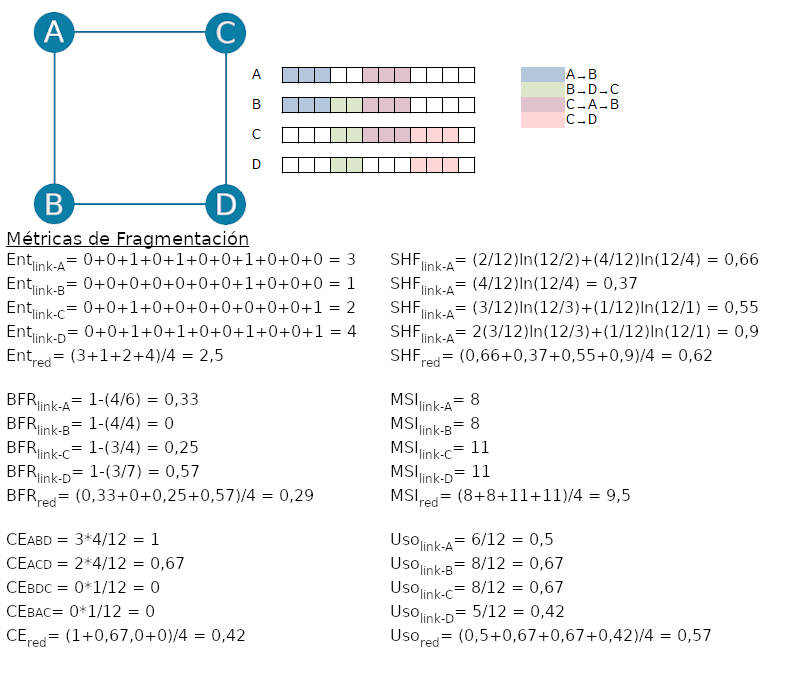
\includegraphics[width=1\textwidth]{capitulos/img/ejemploMetricasCompleto4.png}
    \caption{Ejemplo de métricas de fragmentación}
    \label{fig:ejemploMetricas}
\end{figure}

En la figura \ref{fig:ejemploMetricas} se puede ver un ejemplo de una topología con 4 conexiones activas, el estado de sus enlaces y el cálculo de cada una de las métricas de fragmentación explicadas anteriormente. 

\section{Obtención de datos para el entrenamiento}
Se utilizó un simulador de redes EON \cite{davalos2019spectrum} para la generación del conjunto de datos a ser utilizados para el entrenamiento de la red neuronal.

Para esto se utilizaron dos topologías de red: USNET y NSFNET, en donde por cada topología se realizaron 50 simulaciones con volumen de  tráfico variable en la misma simulación, para lograr que la cantidad de conexiones activas no permanezca constante durante la simulación.  La variación de tráfico usada fue la que se ve en la figura \ref{fig:traficos}-a, el proceso se realizó durante 1210 unidades de tiempo para cada simulación, generando un total de 121.000 registros.

Una vez generados los datos, los mismos fueron preprocesados, de forma a obtener los valores de la probabilidad de bloqueo que deseamos estimar.

El preprocesamiento consiste en el cálculo del índice de bloqueo en base a la ecuación \ref{eq:ecuacion_ib}, donde para un tiempo t, utilizando una ventana de 10 unidades de tiempo hacia delante, para cada instante podemos obtener una mirada hacia delante de posibles bloqueos, \(FSB_{i}\) es la sumatoria de \textit{FS} bloqueados en el tiempo \textit{i} y \(FSD_{i}\) es la sumatoria de \textit{FS} demandados en el tiempo \textit{i}.

\begin{equation} \label{eq:ecuacion_ib}
        PB_{t} = \frac{\sum_{i=t}^{t+T}FSB_{i}}{\sum_{i=t}^{t+T}FSD_{i}}
\end{equation}

Además, una vez separados los datos y debido a la diferencia de rangos de valores, los mismos son normalizados, usando la siguiente fórmula.
\begin{equation}
    n = x - \frac{train_{mean}}{train_{std}}
\end{equation}
Donde x es el valor que queremos normalizar, \(train_{mean}\) la media de valores y \(train_{std}\) es la desviación estándar. 

\begin{figure}
    \centering
    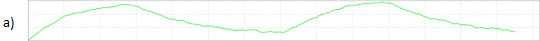
\includegraphics[width=1\textwidth]{capitulos/img/trafico_1_a.png}
    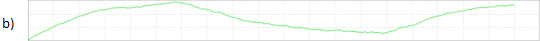
\includegraphics[width=1\textwidth]{capitulos/img/trafico_2_b.png}
    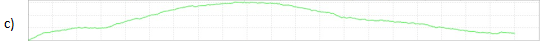
\includegraphics[width=1\textwidth]{capitulos/img/trafico_3_c.png}
    \caption{Volumen de tráfico variado utilizado}
    \label{fig:traficos}
\end{figure}

\section{Herramientas Utilizadas}

En esta sección se presentan las herramientas utilizadas para la implementación del método propuesto en este trabajo, seleccionadas luego de realizar numerosas ejecuciones de prueba para obtener los valores de los parámetros del modelo, asi como la prueba de concepto en sí.

Para todo el proceso de \textit{Machine Learning} se utilizó la plataforma de código abierto llamada \textit{\textbf{TensorFlow}} \cite{tensowFlow} en el lenguaje de programación \textit{\textbf{Python}}. En la creación y entrenamiento de redes neuronales se utilizó la API de alto nivel incluida en la plataforma \textit{\textbf{Tensorflow}} denominada \textit{\textbf{Keras}}, la cual permite la creación de modelos de aprendizaje automático de forma rápida y sencilla.

Elegimos Tensorflow como herramienta principal debido a que es una plataforma de código abierto orientado a \textit{Machine Learning}. Cuenta con un ecosistema completo de herramientas y librerías que facilitan la creación y desarrollo de aplicaciones de aprendizaje automático, además cuenta con una extensa y muy completa documentación.

\section{Modelado}

Para entrenar los datos recolectados se utilizó un modelo con una capa de entrada de 7 neuronas, dos capas ocultas densamente conectadas, cada una con 64 y 32 neuronas respectivamente, y una capa de salida que devuelve un único valor continuo.
Para todas las capas la función de activación utilizada fue la RELU (Ver sección 3.2.2).

\section{Entrenamiento}
Para el entrenamiento del modelo, se creó un conjunto de datos de entrenamiento utilizando el 70\% de los datos recolectados de forma aleatoria.  

El 20\% de los datos de entrenamiento se utilizó como el conjunto de validación. Una técnica utilizada en el procedimiento es el  llamado parada temprana o \textit{Early Stopping}, el cual mediante el monitoreo del rendimiento del entrenamiento nos permite detenernos una vez que el error de validación aumente de forma sostenida, de forma así evitar un sobre entrenamiento.

El modelo se entrena como máximo por 1000 épocas, el cual se detiene automáticamente cuando el valor del error de validación deja de mejorar. La figura \ref{fig:errorEpocas} muestra la evolución del error al pasar las épocas.

Los parámetros comparados son el error de entrenamiento o \textit{Train Error}, el cuál es el error obtenido durante la fase de entrenamiento del modelo y el error de validación o \textit{Val Error}, que se obtiene en la fase de validación.

Por cada época el \textit{Val Error} es comparado con el  \textit{Train Error},esto hasta que se determina que ya no existe mejora, sino que el error de validación se mantiene o aumenta su valor con respecto al punto de parada.


\begin{figure}[H]
    \centering
    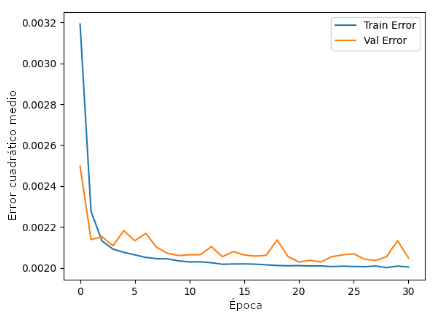
\includegraphics[width=9cm]{capitulos/img/graficoErrorEs.png}
    \caption{Evolución del error a través de épocas}
    \label{fig:errorEpocas}
\end{figure}

\section{Pruebas de predicción}
Para comprobar la efectividad de nuestro modelo se procedió a tomar el 30\% de datos restantes que no fueron incluidos en el entrenamiento y realizar predicciones, como ya conocemos el valor de la probabilidad de bloqueo que se busca predecir podemos calcular el error absoluto medio (MAE) y el error cuadrático medio (MSE). La tabla \ref{table:resultadosPrediccionTabla} muestra los resultados obtenidos, siendo éstos muy satisfactorios.

\begin{table}[H]
\centering
    \caption{Tabla de resultados en pruebas de predicción}
    \begin{tabular}{|l|l|}
        \hline
        MAE & 0.0239 \\ \hline
        MSE & 0.002  \\ \hline
    \end{tabular}
    \label{table:resultadosPrediccionTabla}
\end{table}
\newpage
\begin{figure}[H]
    \centering
    \begin{tabular}{@{}c@{}}
        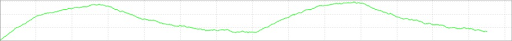
\includegraphics[width=1\textwidth]{capitulos/img/trafico_1.png}\\
        \small (a) Tráfico de volumen variable
    \end{tabular}
    \begin{tabular}{@{}c@{}}
        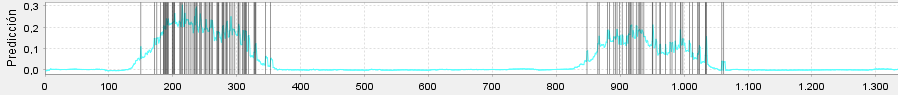
\includegraphics[width=1\textwidth]{capitulos/img/grafico_prediccion_usnet.PNG}\\
        \small (b) Gráfico de valores predichos por la red neuronal
    \end{tabular}
    \caption{Utilización de la red y predicciones}
    \label{fig:utilizacionPredicciones}
\end{figure}
En la Figura \ref{fig:utilizacionPredicciones} - a se observa la variación de la utilización de la red, al realizarse una simulación con volumen de tráfico variable sin realizar procesos de desfragmentación. En la parte b de la misma figura se observa la curva de valores predichos con las técnicas presentadas junto a los bloqueos dados en la misma simulación. Puede observarse cómo este valor acompaña la variación de la utilización de la red, y también toma valores más altos en periodos de tiempo en que la frecuencia de bloqueos se hace más alta. 
